\chapter{Proposed Methods}
% do i need this
% In this chapter, we introduce the proposed methods and experimental methodology. This research aims to address the question, "What would happen if we change the masking strategies?" While numerous strategies have been proposed to enhance the representation of text and images, there has been limited experimentation on altering the masking ratio in masked language modeling (MLM). This study primarily focuses on two main aspects:

% \begin{itemize}
%   \item The referenced model employs masked language modeling to train feature extraction, maintaining a constant masking ratio throughout the training process. This research proposes varying the masking ratio and introducing a time-variant component during training.
%   \item The referenced model includes a function known as momentum-based replace token detection, which also operates with a specific masking ratio. This study examines whether adjusting the masking ratio for this task, similar to the approach taken with MLM, improves prediction performance when both parameters are modified.
% \end{itemize}
%%%
% \color{WIP}
% The purpose of this experiment is to examine the hypothesis that time variant masking ratio affect the prediction on text based person retrieval.
% This is carried out by investigating the relation and sensitivity aware representation learning \cite{Bai2023RaSaRA} that investigated the better representation learning for image and text inputs by detecting the replaced tokens from the converted text and corresponding image inputs. The results showed significant improvements in prediction performance. To investigate further towards the masking ratio, \cite{wettig-etal-2023-mask} investigated that larger models should adopt a higher masking rate rather than masking 15\% of tokens conventionally. Another method from Dongjie Yang, et al, \cite{yang2023learningbettermaskingbetter} proposed time-variant masking ratio decay strategy and POS-tagging weighed masking. In results, the time variant masking decay method outperformed the time invariant masking ratio for F1 score on SQuAD performance during pre-training on BERT-large model. 

The purpose of this experiment is to examine the hypothesis that a time-variant masking ratio affects the prediction accuracy in text-based person retrieval tasks. We approach this by exploring the relationship between the sensitivity-aware representation learning, as investigated by Bai et al. (\cite{Bai2023RaSaRA}) in their work "RaSa," which focuses on improving representation learning for image and text inputs by detecting replaced tokens from the combined text and image inputs. Their results demonstrated significant improvements in prediction performance.

To delve deeper into the impact of masking ratios, (\cite{wettig-etal-2023-mask}) suggested that larger models benefit from adopting a higher masking rate rather than the  conventional 15\% of tokens. Additionally, (\cite{yang2023learningbettermaskingbetter}) proposed a time-variant masking ratio decay strategy along with POS-tagging weighted masking. Their findings indicated that the time-variant masking decay method significantly outperformed the time-invariant masking ratio in terms of F1 score on the SQuAD dataset during the pre-training of the BERT-large model.

Our experiment aims to build on these insights by evaluating the effects of different masking strategies on the performance of vision-language models, specifically in the context of text-based person retrieval. By systematically varying the masking ratio and employing time-variant masking techniques, we seek to determine the optimal approach for enhancing the alignment and interpretation of textual and visual data.

In this experiment, we investigate the effect of the performance towards the time variant masking ratio on replaced token detection task. To evaluate the performance, we will compute the feature similarity score for all image-text pairs. Then we take top-$k$ candidates and calculate their ITM score $s_{itm}$ for ranking. 

\section{Dataset}

\begin{figure}[htbp]
  \begin{center}
      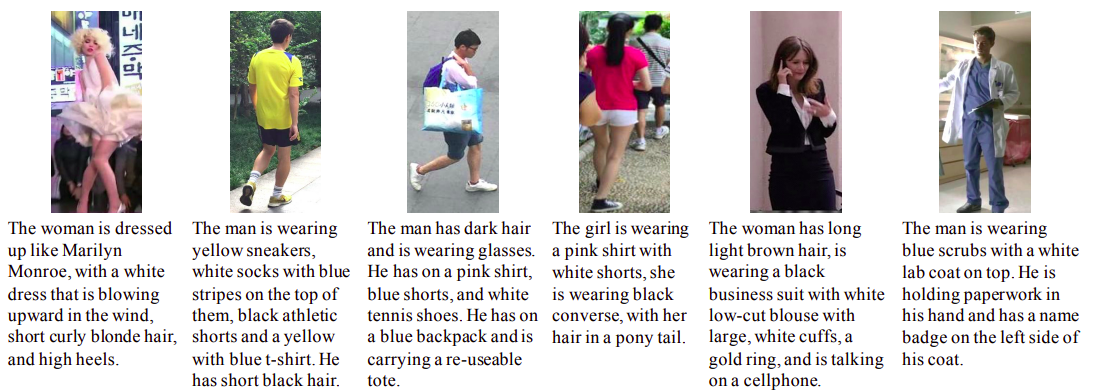
\includegraphics[width=\linewidth]{img/cuhk_pedes.png}
      \caption{Example sentence with corresponding image}
      \label{fig:cuhk_pedes}
  \end{center}
\end{figure}


Dataset we are using is CUHK-PEDES \cite{li2017personsearchnaturallanguage}. This is a large-scale dataset created to facilitate person search using natural language descriptions. It addresses the need for a dataset where persons are described in detail using natural language, enabling practical applications such as video surveillance. Key features of the dataset are shown as follows:
\begin{itemize}
  \item Large-scale: Dataset contains 40,206 images over 13,003 persons 
  \item Annotations: Each images is described with two sentences by independent annotators, in total of 80,412 sentence descriptions
  \item Source diversity: Images are sourced from a variety of existing person re-identification datasets, including CUHK03\cite{li2014deepreid}, Market-1501\cite{7410490}, SSM\cite{ssm}, VIPeR\cite{viper}, and CUHK01\cite{li2012human}.
\end{itemize}

The datasets contains image and corresponding natural language description as shown in Fig\ref{fig:cuhk_pedes}. Image source for CUHK-PEDES are from CUHK03, Market-1501, SSM, VIPER, and CUHK01. The annotations for each image are done by Amazon Mechanical Turk(AMT), which is a crowd workers that are employed to describe each image with two sentence. Each sentence include rich descriptions about person appearance, action poses, and interactions.


\section{Methods}
In this section, we introduce the experimental methods designed to evaluate the performance of vision-language models (VLMs). Recent state-of-the-art VLMs, such as the one described by Bai et al. (2023) in their work "RaSa," utilize an attention mechanism to extract and align features from both images and text using cross-modality encoders. Achieving optimal results necessitates not only robust feature extraction but also the development of sophisticated textual representations to enhance the interpretation of visual data. Therefore, our objective is to train the visual-language model (Bai et al., 2023) by employing diverse strategies for textual information representation. Specifically, we will investigate two distinct methods to determine their impact on model performance.

% explain about the parameters based on the model image and loss function

\section{Masking ratio for masked language modeling} 

\subsection{Introduction}
% explanation about what we do with masking ratio
In natural language pre-training, masked language modeling is utilized to understand the context of an input sentence. This same task is applied to recent vision-language models, where the masked token is predicted using both the image and the remaining text information. Although this method can yield good performance, the typical ratio for masking words in a sentence is fixed at 15\%. In our study, we aim to identify the optimal masking ratio by experimenting with time-invariant masking ratios ranging from 15\% to 40\%. Additionally, we will explore time-variant masking strategies based on previous findings to further enhance model performance.

\subsection{Procedure}

% - モデルとパラメータの具体的な説明
% - 始めにどの比率が効果的かの検証
% - 次に時間変動での検証

We will train the model with constant masking ratio with range of 15\% to 40\% by 5\% steps with the dataset of CUHK-PEDES. Then, from the results, we will take the most highest mAP from the constant masking ratio and use that value with the minimum masking ratio. The minimum ratio will be 2\% since 0\% masking ratio will not train at all. 
Time variant strategy will have the cosine curve and linear curve to see the result. The time variant will have four different methods, linear increase, linear decrease, cosine increase, and cosine decrease. The equations are shown as follows:

\begin{displaymath}
  M_{linear increase}(t) = P*t/T \
  M_{linear decrease}(t) = P*(1-t/T) \
  M_{cosine increase}(t) = P*(1-cos(\pi*t/T)) + 0.02 \ 
  M_{cosine decrease}(t) = P*(1+cos(\pi*t/T)) + 0.02 
\end{displaymath}

For all training tasks, the number of epochs is set to 30, batch size is 13. With this, the model will train under 30 iterations and trains with the dataset which is divided to 13 different datasets. The optimization methods are adamW, learning rate is set to 1.0e-4 at first and create a cosine curve to decrease to 1.0e-5.



% explanation about what strategy we try to experiment
- what we are changing  explanation of parameter
- evaluation method for experiment
- the effect of the experiment 


\section{masking ratio for replaced token detection}
RaSa utilizes this to create a task called sensitivity aware learning.
Sensitivity aware aims to make the model sensitive to specific transformations in the data, particularly textual changes. While many models aim to learn invariant representations that are robust to various data augmentations, RaSa takes it further by encouraging the model to detect and respond to sensitive transformations, such as word replacements in text. This is done using a Momentum-based Replaced Token Detection (M-RTD) task, where the model learns to detect whether a token in the text has been replaced. This sensitivity to changes enhances the robustness and discrimination power of the representations learned by the model.


Predicting more means the model learns from more training signals, so higher prediction rates boost the model performance. From another perspective, each prediction at each masked token leads to a loss gradient, which is averaged to optimize the weights of the model. Averaging across more predictions has a similar effect to increasing the batch size, which is proved to be beneficial for pre-training (Liu et al., 2019). 


corruption rate how much we mask the words from the text
prediction rate how much we predict the mask token 


what i did 
- change the mask 
- visualize the attention section

The structure of the algorithm is done as follows. 
- image encoder
  mlp 
- text encoder
  bert 

When we work on fine tuning, we change the masking ratio on the mlm process. 
the masking ratio will be changed as follows.
flat 
cosine curve 
random 

from these papers, bert scored higher accuracies when using 40\% on masking ratio. This is basically done in text information, 
so we would like to try it out in text based image retireval tasks. T

flat and cosine will work on the range of 40\% and 60\% 
the previous work has been done as 15\%, so we would compare the results with that for the discussion 

\section{Requirements specification}

- model
rasa

- dataset 
CUHK-dataset
ICFG-dataset

- epoch
30

- learning rate 
1e-5 to 1e-6

\section{Attention visualization}
To be able to see where the model is paying attention to, we would use the attention matrix in cross atttention module.



\section{Algorithm implementation}

for the 